% !TeX root = ../main.tex

\section{Methodology}\label{sec:3}

Many factors can influence model performance, including encoder structure, depth and width of layers, and batch size. This thesis investigates the effects of these factors on model performance, particularly the performance of models trained on graph data via self-supervised learning. 

Next, we introduce our experiment settings, including the datasets, data augmentation methods, hyperparameters in the training procedure, and self-supervised learning methods we use for model training.


\subsection{Dataset}


We mainly use the following datasets for model training: MUTAG, NCI1, PROTEINS, and DD. These datasets are collected by TUDataset \cite{tudataset} and are widely used in graph representation learning for evaluating model performance \cite{benchmarking}. 

These datasets contain graph data falling into two categories: chemical molecules and bioinformatics. In MUTAG \cite{mutag} and NCI1 \cite{nci1}, each graph is used to represent a chemical compound or molecule. Each node represents an atom, and each edge represents a chemical bond connecting two nodes. Both datasets are collected for binary graph classification tasks encoded by a one-hot encoding. The prediction task of MUTAG is to predict the mutagenicity of \textit{Salmonella typhimurium}, and the task of NCI1 is to determine whether a chemical compound is positive or negative for cell lung cancer.


On the other hand, in PROTEINS \cite{proteins} and DD \cite{proteins}, each graph is used to represent a protein structure. Each node represents an amino acid, and two nodes are connected by an edge if their distance is less than 6 angstroms apart. The prediction tasks of both datasets are to classify protein structures as enzymes or non-enzymes.


Table \ref{tab:dataset} provides the statistical details of these datasets.


\begin{table}[!htbp]
\centering
\begin{adjustwidth}{-.5in}{-.5in}  
\begin{tabular}{l|c|c|c|c|c}
\toprule
Dataset & Category & \# Graphs & \# Classes & Avg. Nodes & Avg. Edges \\ 
\midrule
MUTAG \cite{mutag} & Molecules & 188 & 	2	&17.93&	19.79 \\
NCI1 \cite{nci1} & Molecules & 4110	&2&	29.87&	32.30 \\
\midrule
PROTEINS \cite{proteins} & Bioinformatics & 1113	&2	&39.06&	72.82 \\
DD \cite{proteins} & Bioinformatics & 1178&	2	&284.32&	715.66 \\
\bottomrule
\end{tabular}
\end{adjustwidth}
\vspace{0.5cm}
\caption[Statistics of datasets]{\textbf{Statistics of datasets.} Incidentally, these datasets are collected for graph classification tasks. }
		\label{tab:dataset}
	
	
	\end{table}
%%%%%%%%%%%%%%%%%%%%%%%%%%%%%%%%%%%%%%%%%%%%%%%%%%%%%%%%%%%%%%%%
%%%%%%%%%%%%%%%%%%%%%%%%%%%%%%%%%%%%%%%%%%%%%%%%%%%%%%%%%%%%%%%%
%%%%%%%%%%%%%%%%%%%%%%%%%%%%%%%%%%%%%%%%%%%%%%%%%%%%%%%%%%%%%%%%


	
\subsection{Data Augmentation}

Self-supervised learning heavily relies on data augmentation for model training \cite{ding2022data, zhao2022graph}. Designing a robust and useful augmentation method is an imperative task in the preprocessing stage. Unlike image data, which can be augmented using methods such as random cropping, blurring, or rotation, graph data are subject to different mechanisms for augmentation. Based on GraphCL, we adopt the following four methods for augmenting our graph data:


\textbf{\uppercase{attribute masking.}} This operator replaces an original attribute with a random value generated by a normal distribution. Generally, some nodes have unique attributes. For example, an atom has its chemical property. We expect that a small change in a few nodes' attributes should not affect the information of the graph. 
		
\textbf{\uppercase{node dropping.}} This operator randomly drops some nodes and their linked edges that connect to other nodes. For example, if we set the augmentation ratio to $0.3$, a total of 30\% of the nodes and their connected edges will be dropped. Despite a few nodes being ignored, we expect the hidden information and features of the graph not to be significantly affected.	

\textbf{\uppercase{edge perturbation.}} Similar to the \uppercase{node dropping} operator, this operator randomly adds or deletes an edge based on a specific ratio. We expect that when a few edges between nodes in a graph are perturbed, the hidden property of the graph will be unaffected. 


\textbf{\uppercase{subgraph.}} This operator randomly samples a subgraph from the local part of the raw graph. In general, we expect the information in the graph to be preserved in its partial structure. 


The illustrations for our data augmentation procedures are shown in Figure \ref{fig:aug}, where the red parts drawn in graphs are the output of data augmentation.


\begin{figure}[!htbp]
\centering
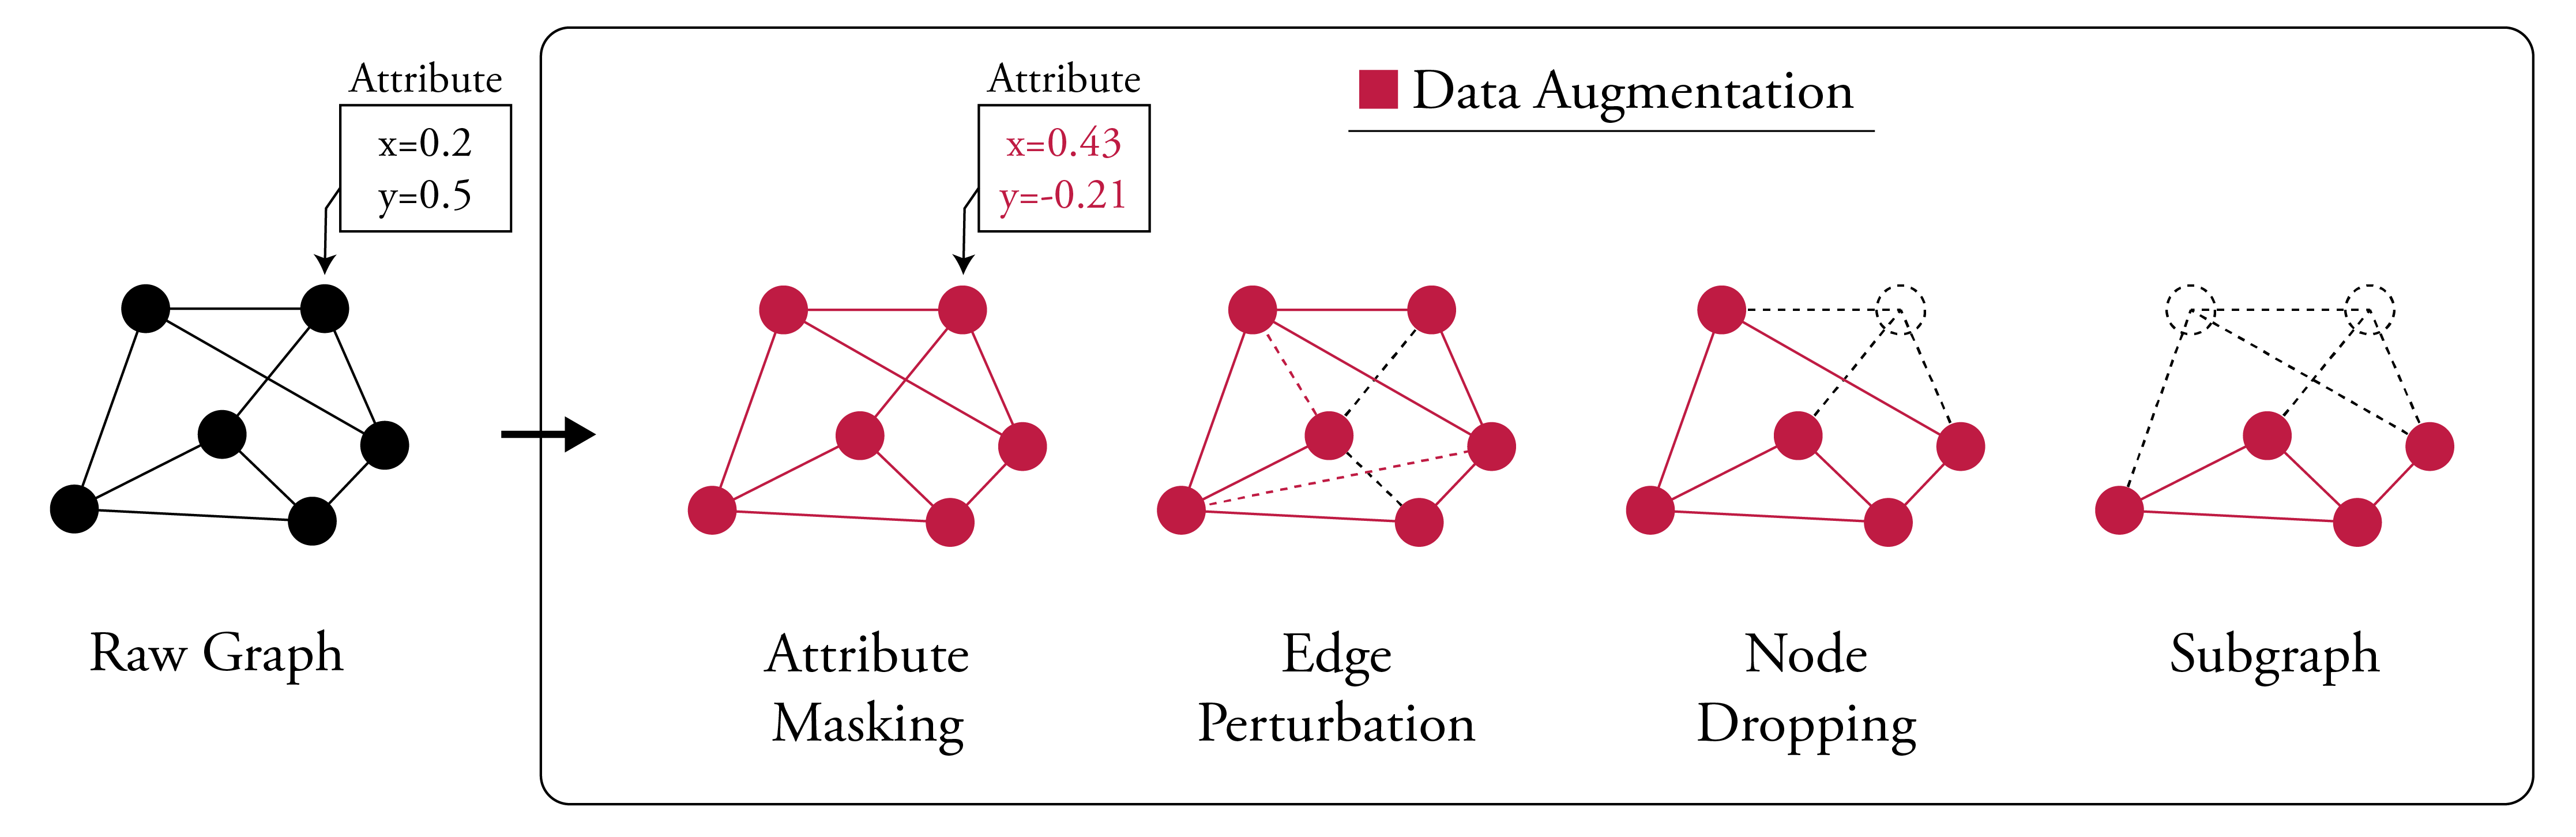
\includegraphics[width=1\textwidth]{./figures/data_augmetation_aka.png}
\vspace{0.5cm}
\caption[Illustrations of augmentation operators]{\textbf{Illustrations of augmentation operators.} Compared with the leftmost raw graph, the red parts drawn in the graphs are the output after data augmentation. The augmented ratio is set to 0.3.}
\label{fig:aug}
\end{figure}


%%%%%%%%%%%%%%%%%%%%%%%%%%%%%%%%%%%%%%%%%%%%%%%%%%%%%%%%%%%%%%%%
%%%%%%%%%%%%%%%%%%%%%%%%%%%%%%%%%%%%%%%%%%%%%%%%%%%%%%%%%%%%%%%%
%%%%%%%%%%%%%%%%%%%%%%%%%%%%%%%%%%%%%%%%%%%%%%%%%%%%%%%%%%%%%%%%



\subsection{Experiment Factor}


To compare the performance of different models trained on graph data, we conducted a series of experiments with varying experiment factors.

We adopted the three self-supervised learning methods, SimCLR, Simsiam, and Barlow Twins, along with the four data augmentations described in Section 3.2, to train our encoders. We set the batch size equal to 64 and 256 (for models trained on the DD dataset, we set the batch size equal to 64 and 128) and the dimension of the hidden space equal to 64 and 512. 


In addition, because the depth of an encoder is a key factor in self-supervised learning, we adopted the monolayer, bilayer, and trilayer architectures for Graph Isomorphism Networks. Because of these experiment settings, there are 144 experiments for each of the four datasets.

These experiment factors are listed in Table \ref{tab:expfactor}. Each experiment was repeated five times to obtain an average result and standard deviation.


\begin{table}[!htbp]
\centering
\begin{adjustwidth}{-.5in}{-.5in}  
\begin{tabular}{r|l}
\toprule
Self-Supervised Approach & \makecell[l]{
~~\llap{\textbullet}~~SimCLR (See Section 3.4 and Figure \ref{fig:arch-simclr}) \\
~~\llap{\textbullet}~~Simsiam (See Section 3.5 and Figure \ref{fig:arch-simsiam})\\
~~\llap{\textbullet}~~Barlow Twins (See Section 3.6 and Figure \ref{fig:arch-bt})} \\
\midrule
Data Augmentation & \makecell[l]{
~~\llap{\textbullet}~~\uppercase{attribute masking}\\
~~\llap{\textbullet}~~\uppercase{edge perturbation} \\
~~\llap{\textbullet}~~\uppercase{node droppping}\\
~~\llap{\textbullet}~~\uppercase{subgraph}\\
~~\llap{\textbullet}~~with ratio 0.3} \\
% \midrule
% Augmentation Ratio & 0.3 \\
\midrule
Mini-batch Size & \makecell[l]{
~~\llap{\textbullet}~~for MUTAG, PROTEINS, NCCI1: 64, 256\\
~~\llap{\textbullet}~~for DD: 64, 128}\\
\midrule
Hidden Dimension & 64, 512\\
\midrule
Encoder & \makecell[l]{~~\llap{\textbullet}~~Encoder Type: Graph Isomorphism Network (GIN)\\
~~\llap{\textbullet}~~Number of Layer: 1 (monolayer), 2 (bilayer), 3 (trilayer)} \\
\midrule
Number of Projector Layer & 3 (trilayer)\\
\midrule
Learning Rate & \makecell[l]{~~\llap{\textbullet}~~0.01\\
~~\llap{\textbullet}~~for Simsiam, with stop-gradient mechanism}\\
\midrule
Epoch  & 200\\
\midrule
Data Proportion & \makecell[l]{
~~\llap{\textbullet}~~ 90\% used in self-supervised for training stage\\
~~\llap{\textbullet}~~ 10\% used in supervised for validation and testing stage}
\\


\bottomrule
\end{tabular}
\end{adjustwidth}
\vspace{0.5cm}
\caption[Detail of experiment factors]{\textbf{Detail of Experiment factors.} The use of different independent and control variables to observe the effect of each factor resulted in 144 experiments being conducted.}
		\label{tab:expfactor}
	\end{table}


%%%%%%%%%%%%%%%%%%%%%%%%%%%%%%%%%%%%%%%%%%%%%%%%%%%%%%%%%%%%%%%%
%%%%%%%%%%%%%%%%%%%%%%%%%%%%%%%%%%%%%%%%%%%%%%%%%%%%%%%%%%%%%%%%
%%%%%%%%%%%%%%%%%%%%%%%%%%%%%%%%%%%%%%%%%%%%%%%%%%%%%%%%%%%%%%%%


\subsection{Contrastive Learning: SimCLR}



Let $\mathbf{x}$ denote the raw data. In SimCLR, we can obtain $\mathbf{x}$'s embedding $\mathbf{h}$ using an encoder $\phi(\cdot)$ and obtain its projection $\mathbf{z}$ through a projector $\theta(\cdot)$. Similarly, we can obtain the augmented embedding $\mathbf{h}^{*}$ and augmented projection $\mathbf{z}^{*}$ using the augmented data $\mathbf{x}^{*}$, where $\mathbf{x}^{*} = \text{AugOperator}(\mathbf{x})$. Mathematically, we can express $\mathbf{h}$ and $\mathbf{z}$ by



\begin{equation}
\mathbf{h}=\phi(\mathbf{x}),
\end{equation}

\begin{equation}
\mathbf{z}=\theta(\mathbf{h})=\theta\Big(\phi(\mathbf{x})\Big), 
\end{equation}

respectively. According to empirical experiments and observation, a projector can make representation more flexible and improve prediction effects.

The loss function used by SimCLR is the NT-Xent loss (normalized temperature-scaled cross entropy loss). For a positive pair of representations $(\mathbf{z},\mathbf{z}^{*})$, the loss function is defined as


\begin{equation}
\mathit{Loss}=-\log\frac{\exp\big(\textbf{sim}(\mathbf{z},\mathbf{z}^{*})/\tau\big)}{\sum^{N}_{\mathbf{z}^{'}\neq\mathbf{z}}\exp\big(\textbf{sim}(\mathbf{z},\mathbf{z}^{'})/\tau)\big)},
\end{equation}

where

\begin{equation}
\textbf{sim}(\mathbf{a},\mathbf{b})=\frac{\mathbf{a}^{\intercal}\mathbf{b}}{\|\mathbf{a}\|_2\|\mathbf{b}\|_2}
\end{equation}

where $\tau$ denotes the trainable temperature parameter and $\textbf{sim}(\mathbf{a},\mathbf{b})$ denotes the $\mathit{l}_2$ normalized cosine similarity between two vectors $\mathbf{a}$ and $\mathbf{b}$. Throughout the experiments, we set $\tau = 0.2$. Notice that the negative representation $\mathbf{z}^{'}$ is generated from the other $N-1$ samples, and the gradient is updated using both the raw and augmented data.

\begin{figure}[!htbp]
% \centering
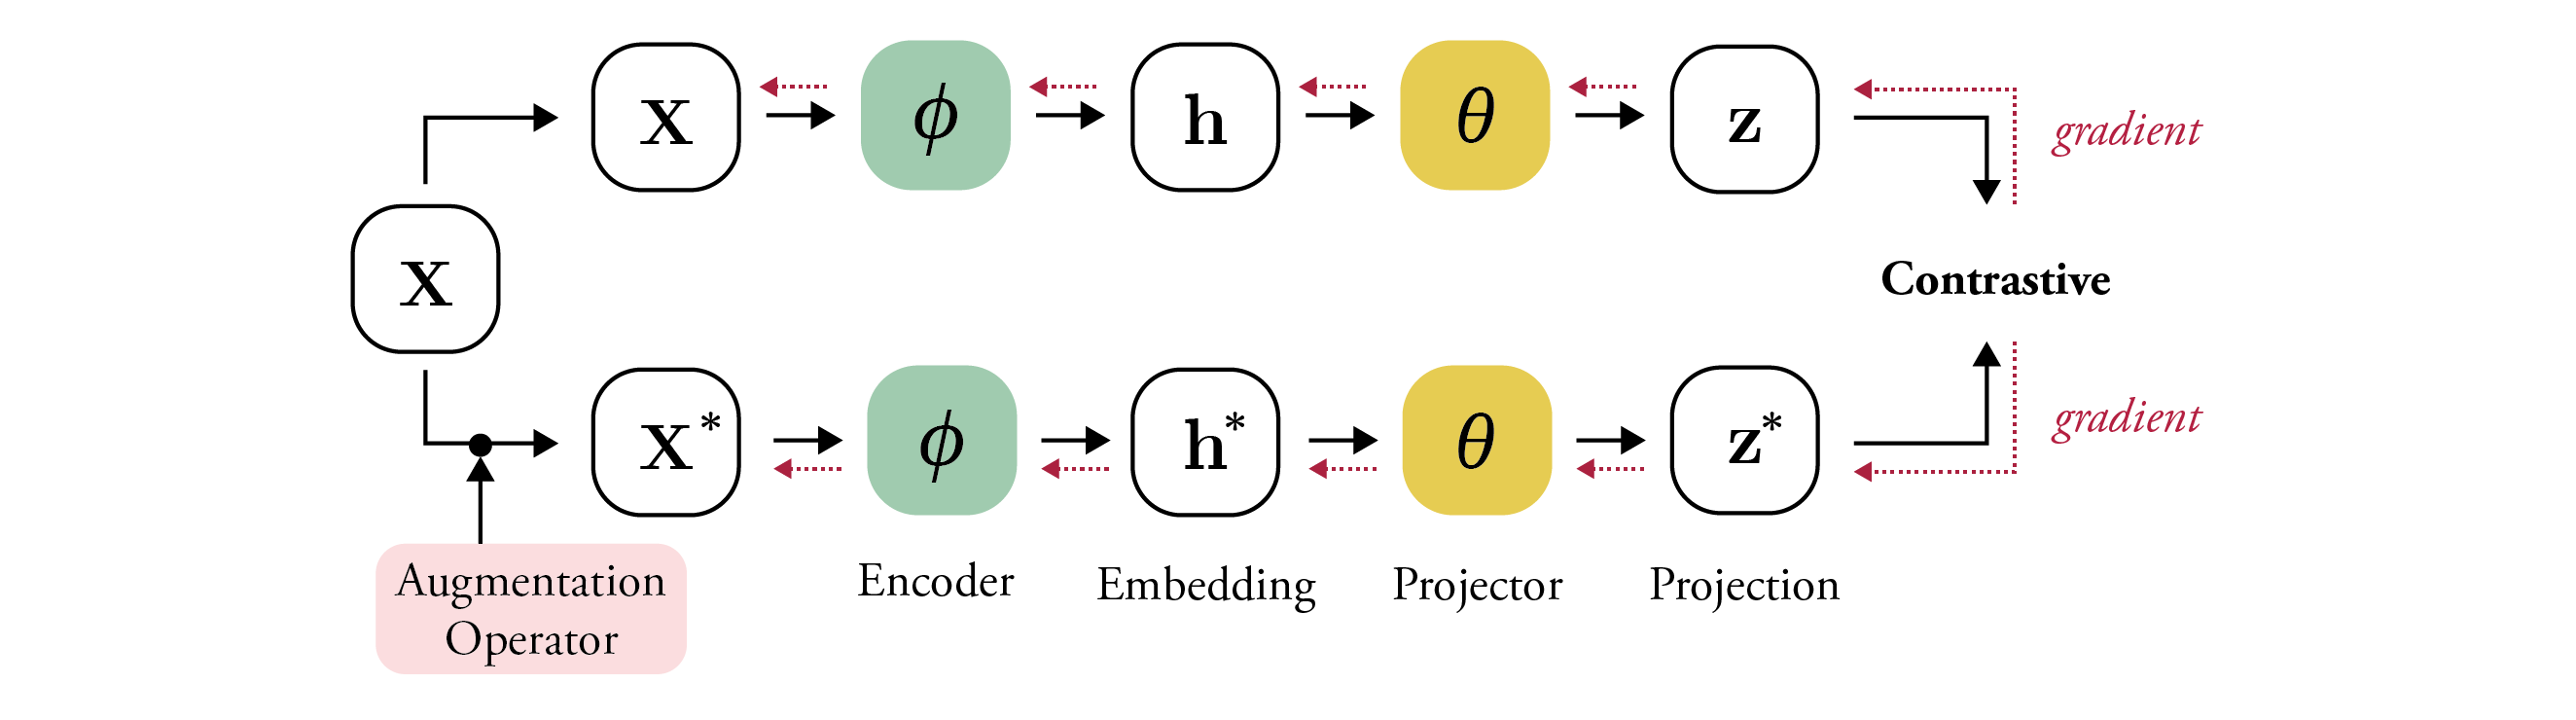
\includegraphics[width=1\textwidth]{./figures/model3_simclr.png}
\vspace{0.5cm}
\caption[Architecture of SimCLR models]{\textbf{Architecture of SimCLR models.} The encoder will learn from the projection of raw and augmented data via NT-Xent loss. According to empirical experiments and observation, a projector can make representation more flexible and improve prediction effects.}
\label{fig:arch-simclr}
\end{figure}


%%%%%%%%%%%%%%%%%%%%%%%%%%%%%%%%%%%%%%%%%%%%%%%%%%%%%%%%%%%%%%%%
%%%%%%%%%%%%%%%%%%%%%%%%%%%%%%%%%%%%%%%%%%%%%%%%%%%%%%%%%%%%%%%%


%%%%%%%%%%%%%%%%%%%%%%%%%%%%%%%%%%%%%%%%%%%%%%%%%%%%%%%%%%%%%%%%


\subsection{Distillation Learning: Simsiam}

In Simsiam, we use an encoder $\phi(\cdot)$ and a projector $\theta(\cdot)$ to obtain the embedding and projection of the raw data $\mathbf{x}$ and the augmented data $\mathbf{x}^{*}$. Moreover, Simsiam introduces a predictor $\psi(\cdot)$ that generates the prediction $\textbf{p}$ via

\begin{equation}
\textbf{p}=\psi(\textbf{z})=\psi(\theta(\mathbf{h}))=\psi\Big(\theta(\phi(\textbf{x}))\Big).\
\end{equation}

The loss function follows the cosine similarity between pairs $(\textbf{z}^{*},\textbf{p})$ and $(\textbf{z},\textbf{p}^{*})$. It is defined by


\begin{equation}
\begin{split}
\mathit{Loss}&=-\frac{1}{2}\sum^{N}_{\text{Dataset}}\Big(\textbf{sim}(\textbf{z}^{*},\textbf{p})+\textbf{sim}(\textbf{z},\textbf{p}^{*})\Big)\\&=-\frac{1}{2}\sum^{N}_{\text{Dataset}}\Big(\frac{(\mathbf{z}^{*})^{\intercal}\mathbf{p}}{\|\mathbf{z}^{*}\|_{2}\|\mathbf{p}\|_{2}}+\frac{\mathbf{z}^{\intercal}\mathbf{p}^{*}}{\|\mathbf{z}\|_{2}\|\mathbf{p}^{*}\|_{2}} \Big).
\end{split}
\end{equation}

To prevent gradient collapse, $\textbf{z}$ and $\textbf{z}^{*}$, the representations produced by the target network, are treated as constants in the training stage. They are subject to the stop-gradient operator when computing the gradient of the loss function. Only $\mathbf{p}$ and $\mathbf{p}^{*}$, the representations produced by the online network, are updated.


As shown in Figure \ref{fig:arch-simsiam}, to calculate the similarity of $(\textbf{z}^{*},\textbf{p})$, Simsiam feeds raw graphs to the online network and augmented graphs to the target network. Thus, only the gradient in the online network is updated via backpropagation. Similarly, when Simsiam calculates the similarity of $(\textbf{z},\textbf{p}^{*})$, it will send raw graphs to the target network and send augmented graphs to the online network.




\begin{figure}[!htbp]
% \centering
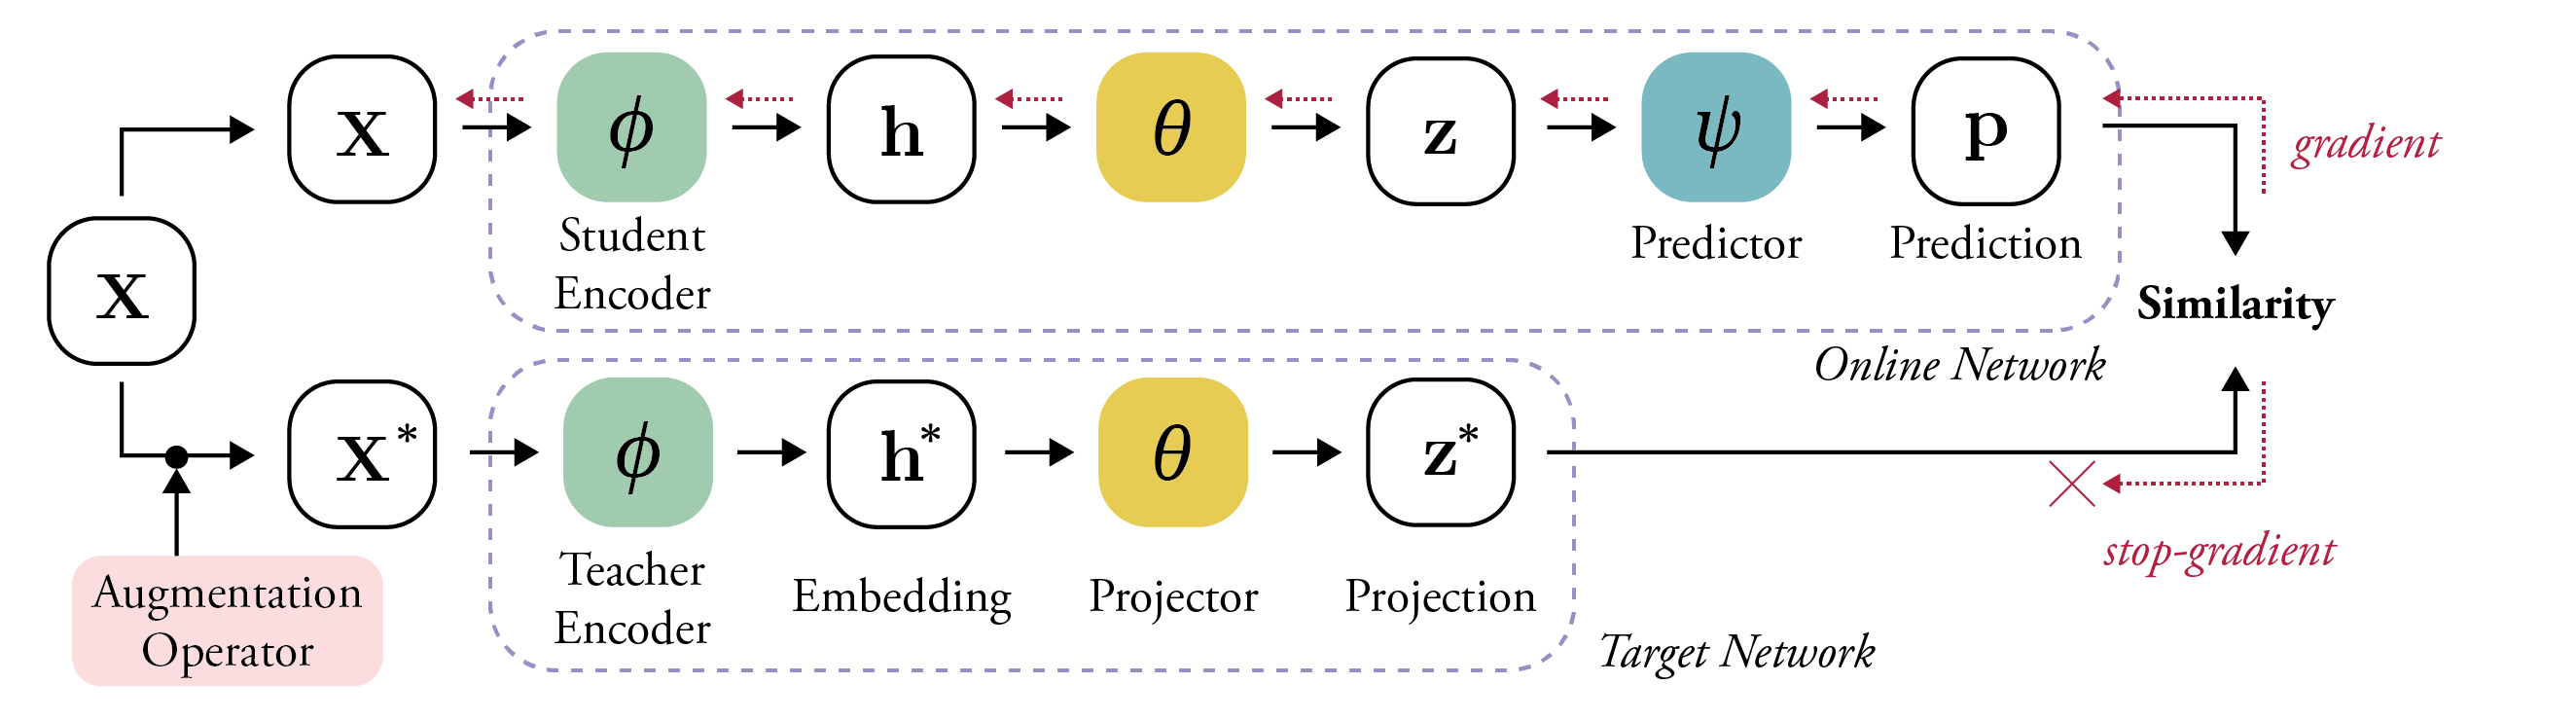
\includegraphics[width=1\textwidth]{./figures/model3_simsiam.png}
\vspace{0.5cm}
\caption[Architecture of Simsiam models]{\textbf{Architecture of Simsiam models.} For example, to calculate the similarity of $(\textbf{z}^{*},\textbf{p})$, Simsiam feeds raw graphs to the online network and augmented graphs to the target network. Only the gradient in the online network is updated via backpropagation.}
\label{fig:arch-simsiam}
\end{figure}



%%%%%%%%%%%%%%%%%%%%%%%%%%%%%%%%%%%%%%%%%%%%%%%%%%%%%%%%%%%%%%%%
%%%%%%%%%%%%%%%%%%%%%%%%%%%%%%%%%%%%%%%%%%%%%%%%%%%%%%%%%%%%%%%%
%%%%%%%%%%%%%%%%%%%%%%%%%%%%%%%%%%%%%%%%%%%%%%%%%%%%%%%%%%%%%%%%


\subsection{Redundancy Reduction: Barlow Twins}

Compared with Simsiam, which uses the projection–prediction pair $\textbf{z}$ and $\textbf{p}^{*}$, Barlow Twins directly uses the embedding pair for comparison. To calculate the loss function, Barlow Twins \cite{bielak2021graph} computes the cross-correlation matrix $\mathcal{C}$ between the outputs of two identical networks along the batch dimension. The $(i,j)$th element of the correlation matrix $\mathcal{C}$ is defined by



\begin{equation}
\mathcal{C}_{ij}=\frac{\sum_b\big((\tilde{\textbf{h}_\textbf{x}})_{b,i}\big)\cdot\big(\tilde{(\textbf{h}_\textbf{x}^{*}})_{b,j}\big)}{\sqrt{\sum_b\big(\tilde{(\textbf{h}_\textbf{x}})_{b,i}\big)}\cdot\sqrt{\sum_b\big(\tilde{(\textbf{h}_\textbf{x}^{*}})_{b,j}\big)}}.
\end{equation}

where $\tilde{\textbf{h}}$ denotes the normalized embedding of $\textbf{h}$ and $\mathcal{C}_{ij}$ should be between $1$ (perfect correlation) and $-1$ (perfect anticorrelation). If two identical networks are the same, known as perfect correlation, the correlation matrix $\mathcal{C}$ should be a diagonal matrix with $1$, a.k.a. an identity matrix $\mathcal{I}$. 

A good encoder should recognize augmentation data as having the same label as raw data. To train this encoder to distinguish a raw graph from an augmented graph and other irrelevant graphs, the loss function is divided into two parts, namely, the invariance term and redundancy reduction term, which are defined by

\begin{equation}
\mathit{Loss}=\underbrace{\sum_i(1-\mathcal{C}_{ii})^2}_{\text{invariance term}}+\lambda\underbrace{\Big(\sum_i\sum_{i\neq j}\mathcal{C}_{ij}^2\Big)}_{\text{{redundancy reduction  term}}},
\end{equation}

respectively. Here, $\lambda$ is a positive constant used to trade off the importance of the invariance term and redundancy reduction term of the loss. 

\begin{figure}[!htbp]
% \centering
{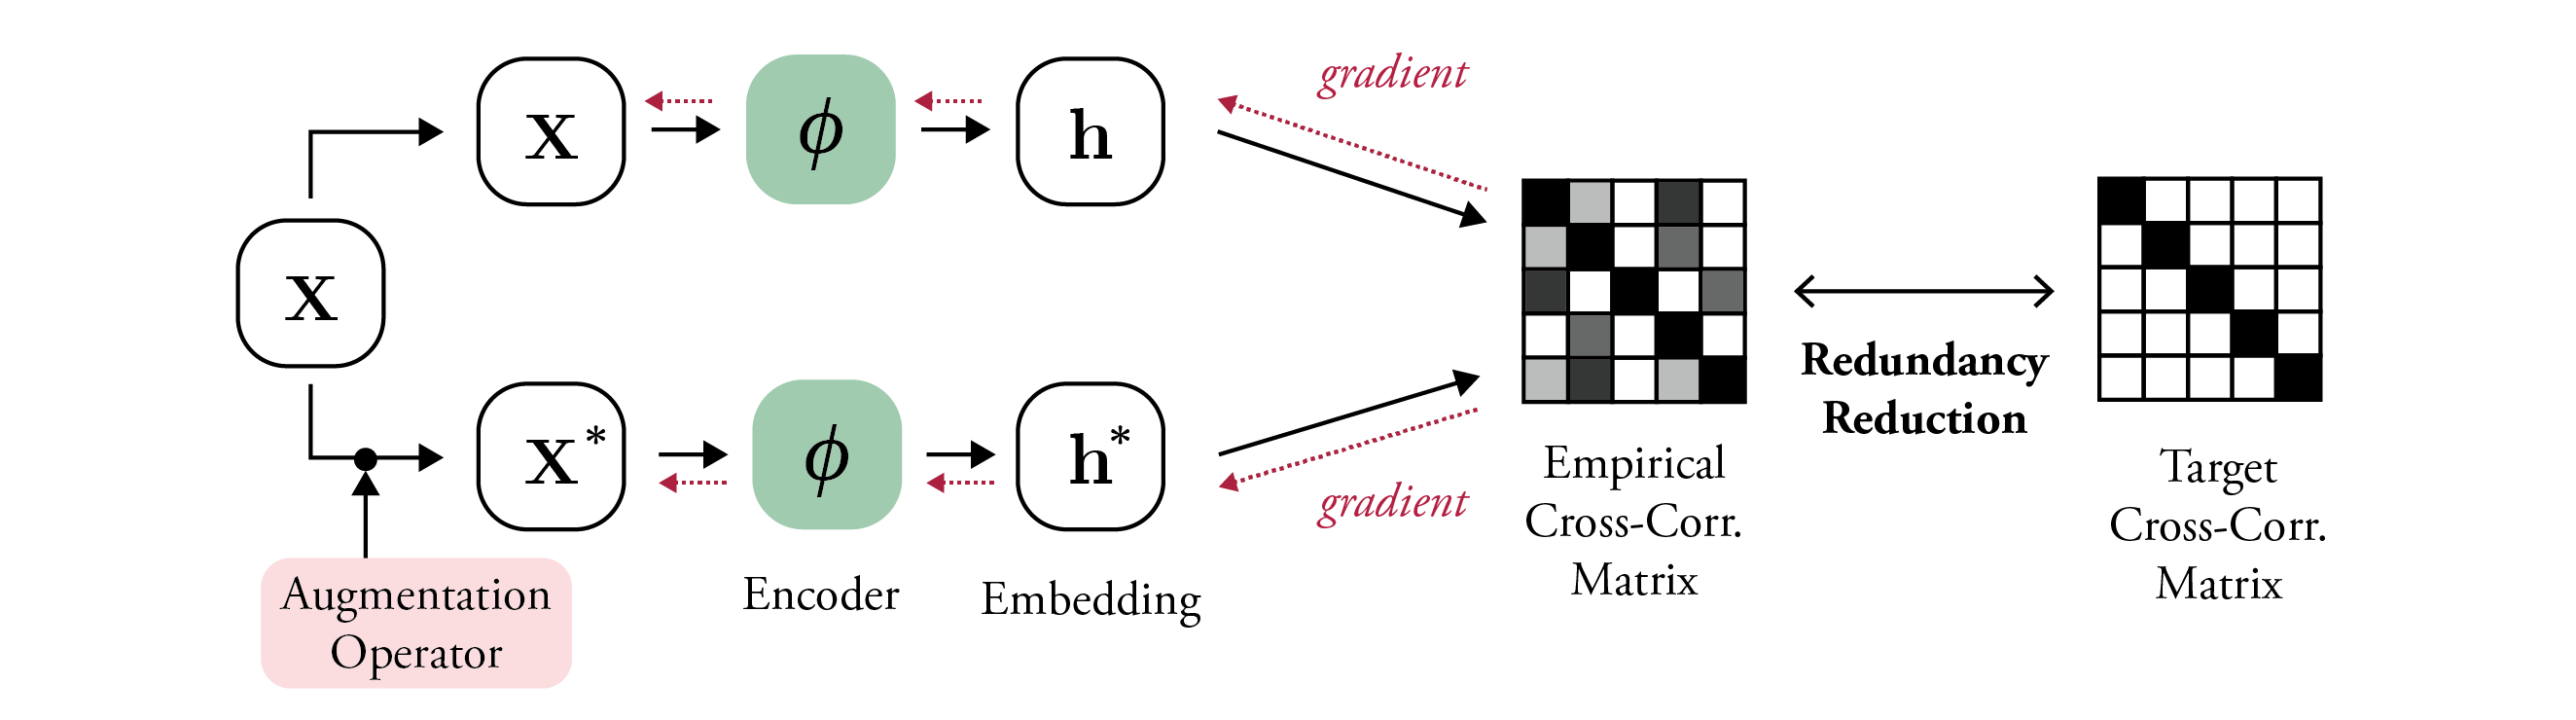
\includegraphics[width=1\textwidth]{./figures/model3_barlowtwins.png}}
\vspace{0.5cm}
\caption[Architecture of Barlow Twins models]{\textbf{Architecture of Barlow Twins models.} The target of an encoder is to classify the embeddings of raw and augmented data as the same label, where the correlation matrix $\mathcal{C}$ of embeddings should be an identity matrix $\mathcal{I}$.}
\label{fig:arch-bt}
\end{figure}






\subsection{Discussion}

In this chapter, we have described four benchmarks that will be used to train the GNNs. We also have described the data augmentation techniques used in model training. Furthermore, we have discussed the three self-supervised learning methods, SimCLR, Simsiam, and Barlow Twins, that will be used to train the GNNs on unlabeled data: contrastive learning, distillation learning, and dimension reduction approach, respectively. 

In the next chapter, we will evaluate the performance of the three self-supervised learning methods by conducting simulation experiments on the four datasets.
